\documentclass[notes]{beamer}
\usepackage{graphicx}
\usepackage{url}
\usepackage[english, portuguese]{babel}
\usepackage[latin1, utf8]{inputenc}
\usepackage{times}
\usepackage[T1]{fontenc}
\usepackage{fancyhdr}
\mode<presentation>


{
  % A tip: pick a theme you like first, and THEN modify the color theme, and then add math content.
  % Warsaw is the theme selected by default in Beamer's installation sample files.

  %%%%%%%%%%%%%%%%%%%%%%%%%%%% THEME
%\usetheme{AnnArbor}
%\usetheme{Antibes}
%\usetheme{Bergen}
%\usetheme{Berkeley}
%\usetheme{Berlin}
% \usetheme{Boadilla}
%\usetheme{boxes}
%\usetheme{CambridgeUS}
%\usetheme{Copenhagen}
%\usetheme{Darmstadt}
 \usetheme{default}
% \usetheme{Dresden}
%\usetheme{Frankfurt}
%\usetheme{Goettingen}
%\usetheme{Hannover}
%\usetheme{Ilmenau}
%\usetheme{JuanLesPins}
%\usetheme{Luebeck}
%\usetheme{Madrid}
% \usetheme{Malmoe}
%\usetheme{Marburg}
%\usetheme{Montpellier}
%\usetheme{PaloAlto}
%\usetheme{Pittsburgh}
%\usetheme{Rochester}
%\usetheme{Singapore}
%\usetheme{Szeged}
%\usetheme{Warsaw}

  %%%%%%%%%%%%%%%%%%%%%%%%%%%% COLOR THEME
  %\usecolortheme{albatross}
  %\usecolortheme{beetle}
  %\usecolortheme{crane}
  %\usecolortheme{default}
  %\usecolortheme{dolphin}
  %\usecolortheme{dove}
  %\usecolortheme{fly}
  %\usecolortheme{lily}
  \usecolortheme{orchid}
  %\usecolortheme{rose}
  %\usecolortheme{seagull}
  %\usecolortheme{seahorse}
  %\usecolortheme{sidebartab}
  %\usecolortheme{structure}
  %\usecolortheme{whale}

  %%%%%%%%%%%%%%%%%%%%%%%%%%%% OUTER THEME
  %\useoutertheme{default}
  %\useoutertheme{infolines}
  %\useoutertheme{miniframes}
  %\useoutertheme{shadow}
  %\useoutertheme{sidebar}
  %\useoutertheme{smoothbars}
  %\useoutertheme{smoothtree}
  %\useoutertheme{split}
  %\useoutertheme{tree}

  %%%%%%%%%%%%%%%%%%%%%%%%%%%% INNER THEME
  %\useinnertheme{circles}
  %\useinnertheme{default}
  %\useinnertheme{inmargin}
  %\useinnertheme{rectangles}
  %\useinnertheme{rounded}

  %%%%%%%%%%%%%%%%%%%%%%%%%%%%%%%%%%%

  \setbeamercovered{transparent} % or whatever (possibly just delete it)
  % To change behavior of \uncover from graying out to totally invisible, can change \setbeamercovered to invisible instead of transparent. apparently there are also 'dynamic' modes that make the amount of graying depend on how long it'll take until the thing is uncovered.

}


% Get rid of nav bar
\beamertemplatenavigationsymbolsempty

% Use short top
\usepackage[headheight=12pt,footheight=12pt]{beamerthemeboxes}
%\addheadboxtemplate{\color{black}}{
%\hskip0.3cm
%\color{white}
\insertshortauthor
%\insertframenumber \ \ \ \ \ \ \ 
%\insertsection \ \ \ \ \ \ \ \ \ \ \ \ \ \ \ \ \  \insertsubsection
%\hskip0.3cm}
%\addheadboxtemplate{\color{black}}{
%\color{white}
%\ \ \ \ 
%\insertsection
%}
%\addheadboxtemplate{\color{black}}{
%\color{white}
%\ \ \ \ 
%\insertsubsection
%}
\title{Measurement and Analysis of Child Pornography Trafficking on P2P Networks\nocite{Hurley}}
\subtitle{}

\def\logounicamp{%
\resizebox{!}{7.5ex}{
\includegraphics{unicamp.pdf}}
}

\def\logoabaco{%
\resizebox{!}{7.5ex}{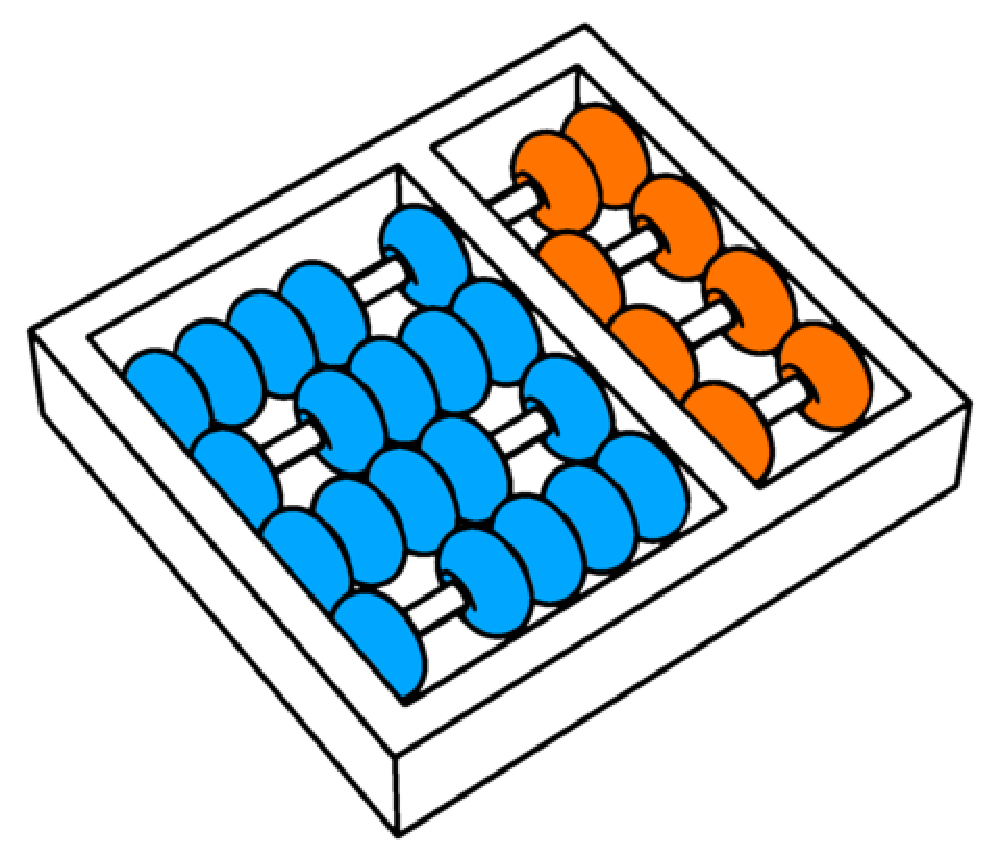
\includegraphics{abaco.pdf}}
}

\institute{Instituto de Computação - Unicamp}

\date{\today}

\subject{Talks}

\def\defn#1{{\color{red} #1}}
% Insere o numero da pagina no rodape.

\setbeamertemplate{headline}[text line]{%
  \parbox{\linewidth}{\vspace*{8pt}\hfill\insertsection}}

\setbeamertemplate{footline}[text line]{%
  \parbox{\linewidth}{\vspace*{-8pt}\logounicamp\hfill\institute\hfill\inserttitle
  \hfill\logoabaco\hfill\insertpagenumber}}
\setbeamertemplate{navigation symbols}{}

\author{Ryan Hurley, Swagatika Prusty, Hamed Soroush, Robert J. Walls
Jeannie Albrecht, Emmanuel Cecchet, Brian Neil Levine
Marc Liberatore, Brian Lynn, Janis Wolak}

\begin{document}

\begin{frame}
  \titlepage
\end{frame}

\begin{frame}
  \frametitle{Scheduling}
  \tableofcontents
\end{frame}

\section{Introduction} 
%este é um slide de exemplo
\begin{frame} %começa um novo slide (frame)

\end{frame}

\section{Criminal Investigation}
\begin{frame}

\begin{itemize} 
    \item[\checkmark] Works properly and is evaluated under the goal of the investigations.
    
    \item[\checkmark] We follow that principles, (basic principles) rather than isolated characterization of the users.
    
    \item[\checkmark] We will review the USA\footnote{Fourth Amendment and related jurisprudence} Law under the constraints of criminal investigations for Children Pornograph.
\end{itemize}

\end{frame}

\begin{frame}
\begin{block}{Works properly and is evaluated under the goal of the investigations}

\begin{itemize}

\item[\checkmark]That  means: The criminal investigation is increasingly advanced and with more development tools for this one. 

\item[\checkmark]There are always more groups that works to find and to discover and try to prevent Child Pornography (CP).

\item[\checkmark]But it is very difficult do prevent, because of the large scale growth in the worldwide web. There are over 1,8 milion CP in internet ''found on eMule'' (we estimate much more).

\end{itemize}

\end{block}

\end{frame}

\begin{frame}
\begin{block}{Basic principles rather than isolated characterization of the users}

\begin{itemize}

\item[\checkmark]This means that we will not discuss about a particular user, but the market situation that involves this type of crime.

\item[\checkmark]In criminal investigations of the type we consider search warrants must specify this location, and not a person (not a user).

\item[\checkmark]Actions by the investigators are shortened by law ''Fourth Amendment and Related Jurisprudence'', where this means that the user has a protection on a electronic data.

\end{itemize}

\end{block}

\end{frame}

\begin{frame}
\begin{block}{What is wrong with Fourth Amendment Jurisprudence?}

\textbf{The Third Party Doctrine}
 
According to the Supreme Court's third party doctrine, personal information, once exposed to any third party, loses all Fourth Amendment protection. Some information exposed to third parties is protected by various statutes, but those can be inconsistent and outdated. The Electronic Communications Privacy Act (ECPA), for example, is notably out of date, leaving privacy protection of technology, as the Ninth Circuit put it, ''a confusing and uncertain area of the law.''. Some privacy interests that are currently unprotected under the Fourth Amendment. Konop ... also receive protection under the First Amendment – but that protection is far from comprehensive... (1967)

\end{block}

\end{frame}

\begin{frame}

\begin{itemize}

\item[\checkmark]The goal of the pre-warrant phase is not to make an arrest (a user, for example), but it is to obtain a judicially issued search warrant, for such cause (CP).

\item[\checkmark]This means, that we will look for a specify location, and not a person.

\item[\checkmark]Arrests in these criminal cases are typically not based on the network-acquired evidence. They are based on the fruits of the search and the person identified as possessing the contraband materials.

\end{itemize}

\end{frame}

\begin{frame}

\begin{itemize}

\item[\checkmark]Finally, we note that this follows a forensics model and
not the traditional security attacker model.

\item[\checkmark]The techniques can be applied very successfully even though there exist many ways to defeat them.

\item[\checkmark]But many people do not attempt to hide them, only change the name of the file, as we know to hide the word ''sexually'', but a intentionally name to be ease to discover the file for another peer.

\end{itemize}

\end{frame}

\section{Forensic Measurement}
\begin{frame}

\end{frame}

\section{Availability and Resilience}
\begin{frame}

\end{frame}

\section{FOI Redundancy and Availability}
\begin{frame}

\end{frame}

\section{Comparing Aggressive Peers}
\begin{frame}

\begin{itemize}

\item[\checkmark]We know that the strategies for removing content from the entire ecosystem (the internet) must target offenders from all countries.

\item[\checkmark]We do not have of a unified effort, and no such collaboration exists.

\item[\checkmark]Investigators need a triage strategy.

\item[\checkmark]The better were if the investigators have target to catch the more dangerous criminals, but such information is not available.

\end{itemize}

\end{frame}

\begin{frame}

\begin{itemize}

\item[\checkmark]In lieu of that ideal, investigators can take peers that are offensive in the net.

\item[\checkmark]Peers that show evidence the target of the intent the user.

\item[\checkmark]This includes peers that are online for the longest duration.

\item[\checkmark]Peers that share the largest number of ''FOI'' (File of Interest).

\item[\checkmark]Offenders by P2P network, as we know: eMule, Gnutella...or offender that seek to escape detection with the use of TOR.

\end{itemize}

\end{frame}

\begin{frame}

\begin{block}{There are 6 (six) sub-groups of peers offenders:}

\begin{enumerate}

\item The top 10\% of GUID’s of largest corpora.

\item The top 10\% of GUID’s of sharing FOI the most numbers of days.

\item The top 10\% of GUID’s ranked contribuition metric (the same we saw in last topics).

\item The top 10\% of the set of GUID’s linked by ip adress sharing FOI.

\item The top 10\% of GUID’s that use a know TOR exit node.

\item The top 10\% of GUID’s  sharing FOI that use a IP adrres and we infer that is a non TOR relay.

\end{enumerate}

\end{block}

\end{frame}

\begin{frame}
\begin{block}{We can see this  result under the table:}

\begin{table} 

\centering

\caption{Sizes of each GUID subgroup} 

\begin{tabular}{ccc}

\hline 

Identifier & Gnutella & eMule \\ 

\hline
\hline
All GUIDs & 775,941 & 1,895,804 \\
Multi-Networks GUIDs & 84,925 (11\%) & 147,904 (7,8\%) \\
TOR GUIDs & 3,666 (0.47\%) & 16,290 (0.86\%) \\
TOR GUIDs (>2 days) & 2,592 (0.33\%) & 11,998 (0.63\%) \\
Relayed GUIDs & 76,478 (9.9\%) & 78,223 (4.1\%) \\
Top 10\% Observed & 84,235 (11\%) & 190,797 (10\%) \\
Top 10\% by Corpus & 77,782 (10\%) & 189,951 (10\%) \\
Top 10\% by Contribution & 77,595 (10\%) & 189,581 (10\%)\\

\hline
\end{tabular}
\label{table2}
\end{table} 

\end{block}

\end{frame}

\section{Analysis of User Aliasing}
\begin{frame}

\end{frame}

\section{Measurement Limitations}
\begin{frame}

\end{frame}

\section{Related Work}
\begin{frame}

\end{frame}

\section{Conclusions and Future Work}
\begin{frame}

\end{frame}

\section{References}
\begin{frame} %%[allowframebreaks]

\frametitle{Bibliography}

\bibliographystyle{unsrt}
\bibliography{refs}

\end{frame}

%%%%% Thanks page
\begin{frame}
\frametitle{Thanks}
\vskip20pt

\begin{center}
{\bf \color{alert} Thanks!}
\end{center}

\vskip20pt

\begin{center}

\vskip12pt
\end{center}

\titlepage
\end{frame}

\end{document}